\begin{tikzpicture}[scale=.2, anchor=west]
\node[draw opacity=0, fill opacity=0, anchor=south west] (dummyL) at (-3, -15){};
\node[draw=black, rectangle split, anchor=south west, rectangle split parts=3] (sn0xb34040) at ([xshift=2cm]dummyL){
\begin{tikzpicture}[scale=.2]
\node[circle, scale=0.75, fill] (tid0) at (3.75,0){};
\node[circle, scale=0.75, fill] (tid1) at (3,1.5){};
\node[circle, scale=0.75, fill] (tid3) at (1.5,3){};
\node[circle, scale=0.75, fill, red] (tid7) at (0.75,4.5){};
\node[circle, scale=0.75, fill, red] (tid8) at (2.25,4.5){};
\draw[](tid3) -- (tid7);
\draw[](tid3) -- (tid8);
\node[circle, scale=0.75, fill] (tid4) at (3.75,3){};
\node[circle, scale=0.75, fill] (tid5) at (5.25,3){};
\draw[](tid1) -- (tid3);
\draw[](tid1) -- (tid4);
\draw[](tid1) -- (tid5);
\node[circle, scale=0.75, fill] (tid2) at (6.75,1.5){};
\node[circle, scale=0.75, fill, red] (tid6) at (6.75,3){};
\draw[](tid2) -- (tid6);
\draw[](tid0) -- (tid1);
\draw[](tid0) -- (tid2);

\end{tikzpicture}
\nodepart{two}
\footnotesize{5.22068}
\nodepart{three}
\footnotesize{$33\:67$}
};
\node[draw opacity=0, fill opacity=0, anchor=south west] (dummyL) at (-6, -30){};
\node[draw=black, rectangle split, anchor=south west, rectangle split parts=3] (sn0xb36950) at ([xshift=2cm]dummyL){
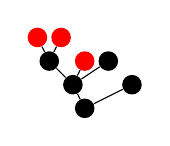
\begin{tikzpicture}[scale=.2]
\node[circle, scale=0.75, fill] (tid0) at (3.75,0){};
\node[circle, scale=0.75, fill] (tid1) at (3,1.5){};
\node[circle, scale=0.75, fill] (tid3) at (1.5,3){};
\node[circle, scale=0.75, fill, red] (tid6) at (0.75,4.5){};
\node[circle, scale=0.75, fill, red] (tid7) at (2.25,4.5){};
\draw[](tid3) -- (tid6);
\draw[](tid3) -- (tid7);
\node[circle, scale=0.75, fill, red] (tid4) at (3.75,3){};
\node[circle, scale=0.75, fill] (tid5) at (5.25,3){};
\draw[](tid1) -- (tid3);
\draw[](tid1) -- (tid4);
\draw[](tid1) -- (tid5);
\node[circle, scale=0.75, fill] (tid2) at (6.75,1.5){};
\draw[](tid0) -- (tid1);
\draw[](tid0) -- (tid2);

\end{tikzpicture}
\nodepart{two}
\footnotesize{4.96296}
\nodepart{three}
\footnotesize{$33\:67$}
};
\node[draw opacity=0, fill opacity=0, anchor=south west] (dummyL) at (-6, -30){};
\node[draw=black, rectangle split, anchor=south west, rectangle split parts=3] (sn0xb36610) at ([xshift=2cm]sn0xb36950.south east){
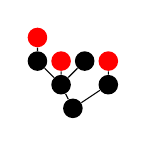
\begin{tikzpicture}[scale=.2]
\node[circle, scale=0.75, fill] (tid0) at (3,0){};
\node[circle, scale=0.75, fill] (tid1) at (2.25,1.5){};
\node[circle, scale=0.75, fill] (tid3) at (0.75,3){};
\node[circle, scale=0.75, fill, red] (tid7) at (0.75,4.5){};
\draw[](tid3) -- (tid7);
\node[circle, scale=0.75, fill, red] (tid4) at (2.25,3){};
\node[circle, scale=0.75, fill] (tid5) at (3.75,3){};
\draw[](tid1) -- (tid3);
\draw[](tid1) -- (tid4);
\draw[](tid1) -- (tid5);
\node[circle, scale=0.75, fill] (tid2) at (5.25,1.5){};
\node[circle, scale=0.75, fill, red] (tid6) at (5.25,3){};
\draw[](tid2) -- (tid6);
\draw[](tid0) -- (tid1);
\draw[](tid0) -- (tid2);

\end{tikzpicture}
\nodepart{two}
\footnotesize{4.84954}
\nodepart{three}
\footnotesize{$33\:33\:33$}
};
\node[draw opacity=0, fill opacity=0, anchor=south west] (dummyL) at (-12, -45){};
\node[draw=black, rectangle split, anchor=south west, rectangle split parts=3] (sn0xb36e20) at ([xshift=2cm]dummyL){
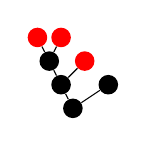
\begin{tikzpicture}[scale=.2]
\node[circle, scale=0.75, fill] (tid0) at (3,0){};
\node[circle, scale=0.75, fill] (tid1) at (2.25,1.5){};
\node[circle, scale=0.75, fill] (tid3) at (1.5,3){};
\node[circle, scale=0.75, fill, red] (tid5) at (0.75,4.5){};
\node[circle, scale=0.75, fill, red] (tid6) at (2.25,4.5){};
\draw[](tid3) -- (tid5);
\draw[](tid3) -- (tid6);
\node[circle, scale=0.75, fill, red] (tid4) at (3.75,3){};
\draw[](tid1) -- (tid3);
\draw[](tid1) -- (tid4);
\node[circle, scale=0.75, fill] (tid2) at (5.25,1.5){};
\draw[](tid0) -- (tid1);
\draw[](tid0) -- (tid2);

\end{tikzpicture}
\nodepart{two}
\footnotesize{4.75926}
\nodepart{three}
\footnotesize{$33\:67$}
};
\node[draw opacity=0, fill opacity=0, anchor=south west] (dummyL) at (-12, -45){};
\node[draw=black, rectangle split, anchor=south west, rectangle split parts=3] (sn0xb36480) at ([xshift=2cm]sn0xb36e20.south east){
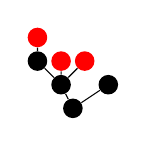
\begin{tikzpicture}[scale=.2]
\node[circle, scale=0.75, fill] (tid0) at (3,0){};
\node[circle, scale=0.75, fill] (tid1) at (2.25,1.5){};
\node[circle, scale=0.75, fill] (tid3) at (0.75,3){};
\node[circle, scale=0.75, fill, red] (tid6) at (0.75,4.5){};
\draw[](tid3) -- (tid6);
\node[circle, scale=0.75, fill, red] (tid4) at (2.25,3){};
\node[circle, scale=0.75, fill, red] (tid5) at (3.75,3){};
\draw[](tid1) -- (tid3);
\draw[](tid1) -- (tid4);
\draw[](tid1) -- (tid5);
\node[circle, scale=0.75, fill] (tid2) at (5.25,1.5){};
\draw[](tid0) -- (tid1);
\draw[](tid0) -- (tid2);

\end{tikzpicture}
\nodepart{two}
\footnotesize{4.56482}
\nodepart{three}
\footnotesize{$67\:33$}
};
\node[draw opacity=0, fill opacity=0, anchor=south west] (dummyL) at (-12, -45){};
\node[draw=black, rectangle split, anchor=south west, rectangle split parts=3] (sn0xb3a170) at ([xshift=2cm]sn0xb36480.south east){
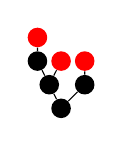
\begin{tikzpicture}[scale=.2]
\node[circle, scale=0.75, fill] (tid0) at (2.25,0){};
\node[circle, scale=0.75, fill] (tid1) at (1.5,1.5){};
\node[circle, scale=0.75, fill] (tid3) at (0.75,3){};
\node[circle, scale=0.75, fill, red] (tid6) at (0.75,4.5){};
\draw[](tid3) -- (tid6);
\node[circle, scale=0.75, fill, red] (tid4) at (2.25,3){};
\draw[](tid1) -- (tid3);
\draw[](tid1) -- (tid4);
\node[circle, scale=0.75, fill] (tid2) at (3.75,1.5){};
\node[circle, scale=0.75, fill, red] (tid5) at (3.75,3){};
\draw[](tid2) -- (tid5);
\draw[](tid0) -- (tid1);
\draw[](tid0) -- (tid2);

\end{tikzpicture}
\nodepart{two}
\footnotesize{4.61343}
\nodepart{three}
\footnotesize{$33\:33\:33$}
};
\node[draw opacity=0, fill opacity=0, anchor=south west] (dummyL) at (-12, -45){};
\node[draw=black, rectangle split, anchor=south west, rectangle split parts=3] (sn0xb39560) at ([xshift=2cm]sn0xb3a170.south east){
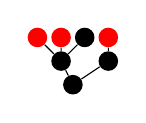
\begin{tikzpicture}[scale=.2]
\node[circle, scale=0.75, fill] (tid0) at (3,0){};
\node[circle, scale=0.75, fill] (tid1) at (2.25,1.5){};
\node[circle, scale=0.75, fill, red] (tid3) at (0.75,3){};
\node[circle, scale=0.75, fill, red] (tid4) at (2.25,3){};
\node[circle, scale=0.75, fill] (tid5) at (3.75,3){};
\draw[](tid1) -- (tid3);
\draw[](tid1) -- (tid4);
\draw[](tid1) -- (tid5);
\node[circle, scale=0.75, fill] (tid2) at (5.25,1.5){};
\node[circle, scale=0.75, fill, red] (tid6) at (5.25,3){};
\draw[](tid2) -- (tid6);
\draw[](tid0) -- (tid1);
\draw[](tid0) -- (tid2);

\end{tikzpicture}
\nodepart{two}
\footnotesize{4.37037}
\nodepart{three}
\footnotesize{$33\:67$}
};
\node[draw opacity=0, fill opacity=0, anchor=south west] (dummyL) at (-15, -60){};
\node[draw=black, rectangle split, anchor=south west, rectangle split parts=3] (sn0xb37640) at ([xshift=2cm]dummyL){
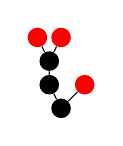
\begin{tikzpicture}[scale=.2]
\node[circle, scale=0.75, fill] (tid0) at (2.25,0){};
\node[circle, scale=0.75, fill] (tid1) at (1.5,1.5){};
\node[circle, scale=0.75, fill] (tid3) at (1.5,3){};
\node[circle, scale=0.75, fill, red] (tid4) at (0.75,4.5){};
\node[circle, scale=0.75, fill, red] (tid5) at (2.25,4.5){};
\draw[](tid3) -- (tid4);
\draw[](tid3) -- (tid5);
\draw[](tid1) -- (tid3);
\node[circle, scale=0.75, fill, red] (tid2) at (3.75,1.5){};
\draw[](tid0) -- (tid1);
\draw[](tid0) -- (tid2);

\end{tikzpicture}
\nodepart{two}
\footnotesize{4.58333}
\nodepart{three}
\footnotesize{$33\:67$}
};
\node[draw opacity=0, fill opacity=0, anchor=south west] (dummyL) at (-15, -60){};
\node[draw=black, rectangle split, anchor=south west, rectangle split parts=3] (sn0xb36010) at ([xshift=2cm]sn0xb37640.south east){
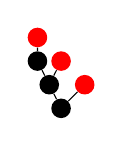
\begin{tikzpicture}[scale=.2]
\node[circle, scale=0.75, fill] (tid0) at (2.25,0){};
\node[circle, scale=0.75, fill] (tid1) at (1.5,1.5){};
\node[circle, scale=0.75, fill] (tid3) at (0.75,3){};
\node[circle, scale=0.75, fill, red] (tid5) at (0.75,4.5){};
\draw[](tid3) -- (tid5);
\node[circle, scale=0.75, fill, red] (tid4) at (2.25,3){};
\draw[](tid1) -- (tid3);
\draw[](tid1) -- (tid4);
\node[circle, scale=0.75, fill, red] (tid2) at (3.75,1.5){};
\draw[](tid0) -- (tid1);
\draw[](tid0) -- (tid2);

\end{tikzpicture}
\nodepart{two}
\footnotesize{4.34722}
\nodepart{three}
\footnotesize{$33\:33\:33$}
};
\node[draw opacity=0, fill opacity=0, anchor=south west] (dummyL) at (-15, -60){};
\node[draw=black, rectangle split, anchor=south west, rectangle split parts=3] (sn0xb39de0) at ([xshift=2cm]sn0xb36010.south east){
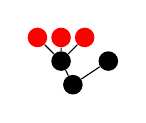
\begin{tikzpicture}[scale=.2]
\node[circle, scale=0.75, fill] (tid0) at (3,0){};
\node[circle, scale=0.75, fill] (tid1) at (2.25,1.5){};
\node[circle, scale=0.75, fill, red] (tid3) at (0.75,3){};
\node[circle, scale=0.75, fill, red] (tid4) at (2.25,3){};
\node[circle, scale=0.75, fill, red] (tid5) at (3.75,3){};
\draw[](tid1) -- (tid3);
\draw[](tid1) -- (tid4);
\draw[](tid1) -- (tid5);
\node[circle, scale=0.75, fill] (tid2) at (5.25,1.5){};
\draw[](tid0) -- (tid1);
\draw[](tid0) -- (tid2);

\end{tikzpicture}
\nodepart{two}
\footnotesize{4}
\nodepart{three}
\footnotesize{$1$}
};
\node[draw opacity=0, fill opacity=0, anchor=south west] (dummyL) at (-15, -60){};
\node[draw=black, rectangle split, anchor=south west, rectangle split parts=3] (sn0xb3a5d0) at ([xshift=2cm]sn0xb39de0.south east){
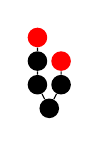
\begin{tikzpicture}[scale=.2]
\node[circle, scale=0.75, fill] (tid0) at (1.5,0){};
\node[circle, scale=0.75, fill] (tid1) at (0.75,1.5){};
\node[circle, scale=0.75, fill] (tid3) at (0.75,3){};
\node[circle, scale=0.75, fill, red] (tid5) at (0.75,4.5){};
\draw[](tid3) -- (tid5);
\draw[](tid1) -- (tid3);
\node[circle, scale=0.75, fill] (tid2) at (2.25,1.5){};
\node[circle, scale=0.75, fill, red] (tid4) at (2.25,3){};
\draw[](tid2) -- (tid4);
\draw[](tid0) -- (tid1);
\draw[](tid0) -- (tid2);

\end{tikzpicture}
\nodepart{two}
\footnotesize{4.4375}
\nodepart{three}
\footnotesize{$50\:50$}
};
\node[draw opacity=0, fill opacity=0, anchor=south west] (dummyL) at (-15, -60){};
\node[draw=black, rectangle split, anchor=south west, rectangle split parts=3] (sn0xb3a370) at ([xshift=2cm]sn0xb3a5d0.south east){
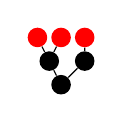
\begin{tikzpicture}[scale=.2]
\node[circle, scale=0.75, fill] (tid0) at (2.25,0){};
\node[circle, scale=0.75, fill] (tid1) at (1.5,1.5){};
\node[circle, scale=0.75, fill, red] (tid3) at (0.75,3){};
\node[circle, scale=0.75, fill, red] (tid4) at (2.25,3){};
\draw[](tid1) -- (tid3);
\draw[](tid1) -- (tid4);
\node[circle, scale=0.75, fill] (tid2) at (3.75,1.5){};
\node[circle, scale=0.75, fill, red] (tid5) at (3.75,3){};
\draw[](tid2) -- (tid5);
\draw[](tid0) -- (tid1);
\draw[](tid0) -- (tid2);

\end{tikzpicture}
\nodepart{two}
\footnotesize{4.05556}
\nodepart{three}
\footnotesize{$33\:67$}
};
\node[draw opacity=0, fill opacity=0, anchor=south west] (dummyL) at (-15, -75){};
\node[draw=black, rectangle split, anchor=south west, rectangle split parts=3] (sn0xb37bd0) at ([xshift=2cm]dummyL){
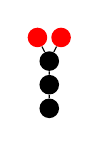
\begin{tikzpicture}[scale=.2]
\node[circle, scale=0.75, fill] (tid0) at (1.5,0){};
\node[circle, scale=0.75, fill] (tid1) at (1.5,1.5){};
\node[circle, scale=0.75, fill] (tid2) at (1.5,3){};
\node[circle, scale=0.75, fill, red] (tid3) at (0.75,4.5){};
\node[circle, scale=0.75, fill, red] (tid4) at (2.25,4.5){};
\draw[](tid2) -- (tid3);
\draw[](tid2) -- (tid4);
\draw[](tid1) -- (tid2);
\draw[](tid0) -- (tid1);

\end{tikzpicture}
\nodepart{two}
\footnotesize{4.5}
\nodepart{three}
\footnotesize{$1$}
};
\node[draw opacity=0, fill opacity=0, anchor=south west] (dummyL) at (-15, -75){};
\node[draw=black, rectangle split, anchor=south west, rectangle split parts=3] (sn0xb37750) at ([xshift=2cm]sn0xb37bd0.south east){
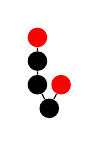
\begin{tikzpicture}[scale=.2]
\node[circle, scale=0.75, fill] (tid0) at (1.5,0){};
\node[circle, scale=0.75, fill] (tid1) at (0.75,1.5){};
\node[circle, scale=0.75, fill] (tid3) at (0.75,3){};
\node[circle, scale=0.75, fill, red] (tid4) at (0.75,4.5){};
\draw[](tid3) -- (tid4);
\draw[](tid1) -- (tid3);
\node[circle, scale=0.75, fill, red] (tid2) at (2.25,1.5){};
\draw[](tid0) -- (tid1);
\draw[](tid0) -- (tid2);

\end{tikzpicture}
\nodepart{two}
\footnotesize{4.125}
\nodepart{three}
\footnotesize{$50\:50$}
};
\node[draw opacity=0, fill opacity=0, anchor=south west] (dummyL) at (-15, -75){};
\node[draw=black, rectangle split, anchor=south west, rectangle split parts=3] (sn0xb38ac0) at ([xshift=2cm]sn0xb37750.south east){
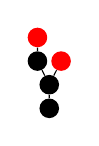
\begin{tikzpicture}[scale=.2]
\node[circle, scale=0.75, fill] (tid0) at (1.5,0){};
\node[circle, scale=0.75, fill] (tid1) at (1.5,1.5){};
\node[circle, scale=0.75, fill] (tid2) at (0.75,3){};
\node[circle, scale=0.75, fill, red] (tid4) at (0.75,4.5){};
\draw[](tid2) -- (tid4);
\node[circle, scale=0.75, fill, red] (tid3) at (2.25,3){};
\draw[](tid1) -- (tid2);
\draw[](tid1) -- (tid3);
\draw[](tid0) -- (tid1);

\end{tikzpicture}
\nodepart{two}
\footnotesize{4.25}
\nodepart{three}
\footnotesize{$50\:50$}
};
\node[draw opacity=0, fill opacity=0, anchor=south west] (dummyL) at (-15, -75){};
\node[draw=black, rectangle split, anchor=south west, rectangle split parts=3] (sn0xb38e80) at ([xshift=2cm]sn0xb38ac0.south east){
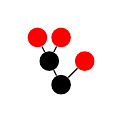
\begin{tikzpicture}[scale=.2]
\node[circle, scale=0.75, fill] (tid0) at (2.25,0){};
\node[circle, scale=0.75, fill] (tid1) at (1.5,1.5){};
\node[circle, scale=0.75, fill, red] (tid3) at (0.75,3){};
\node[circle, scale=0.75, fill, red] (tid4) at (2.25,3){};
\draw[](tid1) -- (tid3);
\draw[](tid1) -- (tid4);
\node[circle, scale=0.75, fill, red] (tid2) at (3.75,1.5){};
\draw[](tid0) -- (tid1);
\draw[](tid0) -- (tid2);

\end{tikzpicture}
\nodepart{two}
\footnotesize{3.66667}
\nodepart{three}
\footnotesize{$67\:33$}
};
\node[draw opacity=0, fill opacity=0, anchor=south west] (dummyL) at (-15, -75){};
\node[draw=black, rectangle split, anchor=south west, rectangle split parts=3] (sn0xb3b350) at ([xshift=2cm]sn0xb38e80.south east){
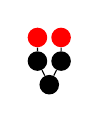
\begin{tikzpicture}[scale=.2]
\node[circle, scale=0.75, fill] (tid0) at (1.5,0){};
\node[circle, scale=0.75, fill] (tid1) at (0.75,1.5){};
\node[circle, scale=0.75, fill, red] (tid3) at (0.75,3){};
\draw[](tid1) -- (tid3);
\node[circle, scale=0.75, fill] (tid2) at (2.25,1.5){};
\node[circle, scale=0.75, fill, red] (tid4) at (2.25,3){};
\draw[](tid2) -- (tid4);
\draw[](tid0) -- (tid1);
\draw[](tid0) -- (tid2);

\end{tikzpicture}
\nodepart{two}
\footnotesize{3.75}
\nodepart{three}
\footnotesize{$1$}
};
\node[draw opacity=0, fill opacity=0, anchor=south west] (dummyL) at (-9, -90){};
\node[draw=black, rectangle split, anchor=south west, rectangle split parts=3] (sn0xb37e70) at ([xshift=2cm]dummyL){
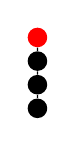
\begin{tikzpicture}[scale=.2]
\node[circle, scale=0.75, fill] (tid0) at (0.75,0){};
\node[circle, scale=0.75, fill] (tid1) at (0.75,1.5){};
\node[circle, scale=0.75, fill] (tid2) at (0.75,3){};
\node[circle, scale=0.75, fill, red] (tid3) at (0.75,4.5){};
\draw[](tid2) -- (tid3);
\draw[](tid1) -- (tid2);
\draw[](tid0) -- (tid1);

\end{tikzpicture}
\nodepart{two}
\footnotesize{4}
\nodepart{three}
\footnotesize{$1$}
};
\node[draw opacity=0, fill opacity=0, anchor=south west] (dummyL) at (-9, -90){};
\node[draw=black, rectangle split, anchor=south west, rectangle split parts=3] (sn0xb38160) at ([xshift=2cm]sn0xb37e70.south east){
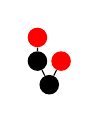
\begin{tikzpicture}[scale=.2]
\node[circle, scale=0.75, fill] (tid0) at (1.5,0){};
\node[circle, scale=0.75, fill] (tid1) at (0.75,1.5){};
\node[circle, scale=0.75, fill, red] (tid3) at (0.75,3){};
\draw[](tid1) -- (tid3);
\node[circle, scale=0.75, fill, red] (tid2) at (2.25,1.5){};
\draw[](tid0) -- (tid1);
\draw[](tid0) -- (tid2);

\end{tikzpicture}
\nodepart{two}
\footnotesize{3.25}
\nodepart{three}
\footnotesize{$50\:50$}
};
\node[draw opacity=0, fill opacity=0, anchor=south west] (dummyL) at (-9, -90){};
\node[draw=black, rectangle split, anchor=south west, rectangle split parts=3] (sn0xb39450) at ([xshift=2cm]sn0xb38160.south east){
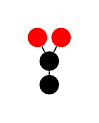
\begin{tikzpicture}[scale=.2]
\node[circle, scale=0.75, fill] (tid0) at (1.5,0){};
\node[circle, scale=0.75, fill] (tid1) at (1.5,1.5){};
\node[circle, scale=0.75, fill, red] (tid2) at (0.75,3){};
\node[circle, scale=0.75, fill, red] (tid3) at (2.25,3){};
\draw[](tid1) -- (tid2);
\draw[](tid1) -- (tid3);
\draw[](tid0) -- (tid1);

\end{tikzpicture}
\nodepart{two}
\footnotesize{3.5}
\nodepart{three}
\footnotesize{$1$}
};
\node[draw opacity=0, fill opacity=0, anchor=south west] (dummyL) at (-6, -105){};
\node[draw=black, rectangle split, anchor=south west, rectangle split parts=3] (sn0xb37f40) at ([xshift=2cm]dummyL){
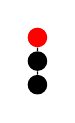
\begin{tikzpicture}[scale=.2]
\node[circle, scale=0.75, fill] (tid0) at (0.75,0){};
\node[circle, scale=0.75, fill] (tid1) at (0.75,1.5){};
\node[circle, scale=0.75, fill, red] (tid2) at (0.75,3){};
\draw[](tid1) -- (tid2);
\draw[](tid0) -- (tid1);

\end{tikzpicture}
\nodepart{two}
\footnotesize{3}
\nodepart{three}
\footnotesize{$1$}
};
\node[draw opacity=0, fill opacity=0, anchor=south west] (dummyL) at (-6, -105){};
\node[draw=black, rectangle split, anchor=south west, rectangle split parts=3] (sn0xb385b0) at ([xshift=2cm]sn0xb37f40.south east){

\begin{tikzpicture}[scale=.2]
\node[circle, scale=0.75, fill] (tid0) at (1.5,0){};
\node[circle, scale=0.75, fill, red] (tid1) at (0.75,1.5){};
\node[circle, scale=0.75, fill, red] (tid2) at (2.25,1.5){};
\draw[](tid0) -- (tid1);
\draw[](tid0) -- (tid2);

\end{tikzpicture}
\nodepart{two}
\footnotesize{2.5}
\nodepart{three}
\footnotesize{$1$}
};
\draw (sn0xb34040.south) -- (sn0xb36950.north);
\draw (sn0xb34040.south) -- (sn0xb36610.north);
\draw (sn0xb36950.south) -- (sn0xb36e20.north);
\draw (sn0xb36950.south) -- (sn0xb36480.north);
\draw (sn0xb36610.south) -- (sn0xb3a170.north);
\draw (sn0xb36610.south) -- (sn0xb36480.north);
\draw (sn0xb36610.south) -- (sn0xb39560.north);
\draw (sn0xb36e20.south) -- (sn0xb37640.north);
\draw (sn0xb36e20.south) -- (sn0xb36010.north);
\draw (sn0xb36480.south) -- (sn0xb36010.north);
\draw (sn0xb36480.south) -- (sn0xb39de0.north);
\draw (sn0xb3a170.south) -- (sn0xb3a5d0.north);
\draw (sn0xb3a170.south) -- (sn0xb36010.north);
\draw (sn0xb3a170.south) -- (sn0xb3a370.north);
\draw (sn0xb39560.south) -- (sn0xb3a370.north);
\draw (sn0xb39560.south) -- (sn0xb39de0.north);
\draw (sn0xb37640.south) -- (sn0xb37bd0.north);
\draw (sn0xb37640.south) -- (sn0xb37750.north);
\draw (sn0xb36010.south) -- (sn0xb38ac0.north);
\draw (sn0xb36010.south) -- (sn0xb37750.north);
\draw (sn0xb36010.south) -- (sn0xb38e80.north);
\draw (sn0xb39de0.south) -- (sn0xb38e80.north);
\draw (sn0xb3a5d0.south) -- (sn0xb37750.north);
\draw (sn0xb3a5d0.south) -- (sn0xb3b350.north);
\draw (sn0xb3a370.south) -- (sn0xb3b350.north);
\draw (sn0xb3a370.south) -- (sn0xb38e80.north);
\draw (sn0xb37bd0.south) -- (sn0xb37e70.north);
\draw (sn0xb37750.south) -- (sn0xb37e70.north);
\draw (sn0xb37750.south) -- (sn0xb38160.north);
\draw (sn0xb38ac0.south) -- (sn0xb37e70.north);
\draw (sn0xb38ac0.south) -- (sn0xb39450.north);
\draw (sn0xb38e80.south) -- (sn0xb39450.north);
\draw (sn0xb38e80.south) -- (sn0xb38160.north);
\draw (sn0xb3b350.south) -- (sn0xb38160.north);
\draw (sn0xb37e70.south) -- (sn0xb37f40.north);
\draw (sn0xb38160.south) -- (sn0xb37f40.north);
\draw (sn0xb38160.south) -- (sn0xb385b0.north);
\draw (sn0xb39450.south) -- (sn0xb37f40.north);
\end{tikzpicture}

%%% Local Variables:
%%% TeX-master: "thesis/thesis.tex"
%%% End: 

\begin{tikzpicture}[scale=.2, anchor=west]
\node[draw opacity=0, fill opacity=0, anchor=south west] (dummyL) at (-3, -15){};
\node[draw=black, rectangle split, anchor=south west, rectangle split parts=3] (sn0xb34100) at ([xshift=2cm]dummyL){
\begin{tikzpicture}[scale=.2]
\node[circle, scale=0.75, fill] (tid0) at (3.75,0){};
\node[circle, scale=0.75, fill] (tid1) at (3,1.5){};
\node[circle, scale=0.75, fill] (tid3) at (1.5,3){};
\node[circle, scale=0.75, fill, red] (tid7) at (0.75,4.5){};
\node[circle, scale=0.75, fill, red] (tid8) at (2.25,4.5){};
\draw[](tid3) -- (tid7);
\draw[](tid3) -- (tid8);
\node[circle, scale=0.75, fill, red] (tid4) at (3.75,3){};
\node[circle, scale=0.75, fill] (tid5) at (5.25,3){};
\draw[](tid1) -- (tid3);
\draw[](tid1) -- (tid4);
\draw[](tid1) -- (tid5);
\node[circle, scale=0.75, fill] (tid2) at (6.75,1.5){};
\node[circle, scale=0.75, fill] (tid6) at (6.75,3){};
\draw[](tid2) -- (tid6);
\draw[](tid0) -- (tid1);
\draw[](tid0) -- (tid2);

\end{tikzpicture}
\nodepart{two}
\footnotesize{5.24126}
\nodepart{three}
\footnotesize{$17\:17\:33\:33$}
};
\node[draw opacity=0, fill opacity=0, anchor=south west] (dummyL) at (-12, -30){};
\node[draw=black, rectangle split, anchor=south west, rectangle split parts=3] (sn0xb3b0e0) at ([xshift=2cm]dummyL){
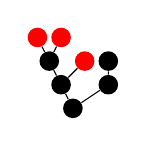
\begin{tikzpicture}[scale=.2]
\node[circle, scale=0.75, fill] (tid0) at (3,0){};
\node[circle, scale=0.75, fill] (tid1) at (2.25,1.5){};
\node[circle, scale=0.75, fill] (tid3) at (1.5,3){};
\node[circle, scale=0.75, fill, red] (tid6) at (0.75,4.5){};
\node[circle, scale=0.75, fill, red] (tid7) at (2.25,4.5){};
\draw[](tid3) -- (tid6);
\draw[](tid3) -- (tid7);
\node[circle, scale=0.75, fill, red] (tid4) at (3.75,3){};
\draw[](tid1) -- (tid3);
\draw[](tid1) -- (tid4);
\node[circle, scale=0.75, fill] (tid2) at (5.25,1.5){};
\node[circle, scale=0.75, fill] (tid5) at (5.25,3){};
\draw[](tid2) -- (tid5);
\draw[](tid0) -- (tid1);
\draw[](tid0) -- (tid2);

\end{tikzpicture}
\nodepart{two}
\footnotesize{5.01543}
\nodepart{three}
\footnotesize{$33\:67$}
};
\node[draw opacity=0, fill opacity=0, anchor=south west] (dummyL) at (-12, -30){};
\node[draw=black, rectangle split, anchor=south west, rectangle split parts=3] (sn0xb3bba0) at ([xshift=2cm]sn0xb3b0e0.south east){
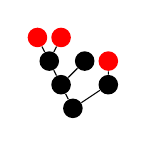
\begin{tikzpicture}[scale=.2]
\node[circle, scale=0.75, fill] (tid0) at (3,0){};
\node[circle, scale=0.75, fill] (tid1) at (2.25,1.5){};
\node[circle, scale=0.75, fill] (tid3) at (1.5,3){};
\node[circle, scale=0.75, fill, red] (tid6) at (0.75,4.5){};
\node[circle, scale=0.75, fill, red] (tid7) at (2.25,4.5){};
\draw[](tid3) -- (tid6);
\draw[](tid3) -- (tid7);
\node[circle, scale=0.75, fill] (tid4) at (3.75,3){};
\draw[](tid1) -- (tid3);
\draw[](tid1) -- (tid4);
\node[circle, scale=0.75, fill] (tid2) at (5.25,1.5){};
\node[circle, scale=0.75, fill, red] (tid5) at (5.25,3){};
\draw[](tid2) -- (tid5);
\draw[](tid0) -- (tid1);
\draw[](tid0) -- (tid2);

\end{tikzpicture}
\nodepart{two}
\footnotesize{4.99537}
\nodepart{three}
\footnotesize{$67\:33$}
};
\node[draw opacity=0, fill opacity=0, anchor=south west] (dummyL) at (-12, -30){};
\node[draw=black, rectangle split, anchor=south west, rectangle split parts=3] (sn0xb3b620) at ([xshift=2cm]sn0xb3bba0.south east){
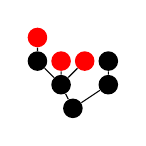
\begin{tikzpicture}[scale=.2]
\node[circle, scale=0.75, fill] (tid0) at (3,0){};
\node[circle, scale=0.75, fill] (tid1) at (2.25,1.5){};
\node[circle, scale=0.75, fill] (tid3) at (0.75,3){};
\node[circle, scale=0.75, fill, red] (tid7) at (0.75,4.5){};
\draw[](tid3) -- (tid7);
\node[circle, scale=0.75, fill, red] (tid4) at (2.25,3){};
\node[circle, scale=0.75, fill, red] (tid5) at (3.75,3){};
\draw[](tid1) -- (tid3);
\draw[](tid1) -- (tid4);
\draw[](tid1) -- (tid5);
\node[circle, scale=0.75, fill] (tid2) at (5.25,1.5){};
\node[circle, scale=0.75, fill] (tid6) at (5.25,3){};
\draw[](tid2) -- (tid6);
\draw[](tid0) -- (tid1);
\draw[](tid0) -- (tid2);

\end{tikzpicture}
\nodepart{two}
\footnotesize{4.86883}
\nodepart{three}
\footnotesize{$67\:17\:17$}
};
\node[draw opacity=0, fill opacity=0, anchor=south west] (dummyL) at (-12, -30){};
\node[draw=black, rectangle split, anchor=south west, rectangle split parts=3] (sn0xb36610) at ([xshift=2cm]sn0xb3b620.south east){
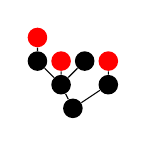
\begin{tikzpicture}[scale=.2]
\node[circle, scale=0.75, fill] (tid0) at (3,0){};
\node[circle, scale=0.75, fill] (tid1) at (2.25,1.5){};
\node[circle, scale=0.75, fill] (tid3) at (0.75,3){};
\node[circle, scale=0.75, fill, red] (tid7) at (0.75,4.5){};
\draw[](tid3) -- (tid7);
\node[circle, scale=0.75, fill, red] (tid4) at (2.25,3){};
\node[circle, scale=0.75, fill] (tid5) at (3.75,3){};
\draw[](tid1) -- (tid3);
\draw[](tid1) -- (tid4);
\draw[](tid1) -- (tid5);
\node[circle, scale=0.75, fill] (tid2) at (5.25,1.5){};
\node[circle, scale=0.75, fill, red] (tid6) at (5.25,3){};
\draw[](tid2) -- (tid6);
\draw[](tid0) -- (tid1);
\draw[](tid0) -- (tid2);

\end{tikzpicture}
\nodepart{two}
\footnotesize{4.84954}
\nodepart{three}
\footnotesize{$33\:33\:33$}
};
\node[draw opacity=0, fill opacity=0, anchor=south west] (dummyL) at (-18, -45){};
\node[draw=black, rectangle split, anchor=south west, rectangle split parts=3] (sn0xb3c5d0) at ([xshift=2cm]dummyL){
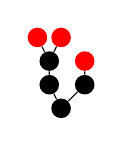
\begin{tikzpicture}[scale=.2]
\node[circle, scale=0.75, fill] (tid0) at (2.25,0){};
\node[circle, scale=0.75, fill] (tid1) at (1.5,1.5){};
\node[circle, scale=0.75, fill] (tid3) at (1.5,3){};
\node[circle, scale=0.75, fill, red] (tid5) at (0.75,4.5){};
\node[circle, scale=0.75, fill, red] (tid6) at (2.25,4.5){};
\draw[](tid3) -- (tid5);
\draw[](tid3) -- (tid6);
\draw[](tid1) -- (tid3);
\node[circle, scale=0.75, fill] (tid2) at (3.75,1.5){};
\node[circle, scale=0.75, fill, red] (tid4) at (3.75,3){};
\draw[](tid2) -- (tid4);
\draw[](tid0) -- (tid1);
\draw[](tid0) -- (tid2);

\end{tikzpicture}
\nodepart{two}
\footnotesize{4.81944}
\nodepart{three}
\footnotesize{$33\:67$}
};
\node[draw opacity=0, fill opacity=0, anchor=south west] (dummyL) at (-18, -45){};
\node[draw=black, rectangle split, anchor=south west, rectangle split parts=3] (sn0xb3a170) at ([xshift=2cm]sn0xb3c5d0.south east){
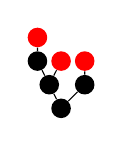
\begin{tikzpicture}[scale=.2]
\node[circle, scale=0.75, fill] (tid0) at (2.25,0){};
\node[circle, scale=0.75, fill] (tid1) at (1.5,1.5){};
\node[circle, scale=0.75, fill] (tid3) at (0.75,3){};
\node[circle, scale=0.75, fill, red] (tid6) at (0.75,4.5){};
\draw[](tid3) -- (tid6);
\node[circle, scale=0.75, fill, red] (tid4) at (2.25,3){};
\draw[](tid1) -- (tid3);
\draw[](tid1) -- (tid4);
\node[circle, scale=0.75, fill] (tid2) at (3.75,1.5){};
\node[circle, scale=0.75, fill, red] (tid5) at (3.75,3){};
\draw[](tid2) -- (tid5);
\draw[](tid0) -- (tid1);
\draw[](tid0) -- (tid2);

\end{tikzpicture}
\nodepart{two}
\footnotesize{4.61343}
\nodepart{three}
\footnotesize{$33\:33\:33$}
};
\node[draw opacity=0, fill opacity=0, anchor=south west] (dummyL) at (-18, -45){};
\node[draw=black, rectangle split, anchor=south west, rectangle split parts=3] (sn0xb36e20) at ([xshift=2cm]sn0xb3a170.south east){
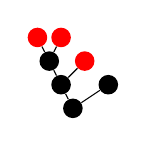
\begin{tikzpicture}[scale=.2]
\node[circle, scale=0.75, fill] (tid0) at (3,0){};
\node[circle, scale=0.75, fill] (tid1) at (2.25,1.5){};
\node[circle, scale=0.75, fill] (tid3) at (1.5,3){};
\node[circle, scale=0.75, fill, red] (tid5) at (0.75,4.5){};
\node[circle, scale=0.75, fill, red] (tid6) at (2.25,4.5){};
\draw[](tid3) -- (tid5);
\draw[](tid3) -- (tid6);
\node[circle, scale=0.75, fill, red] (tid4) at (3.75,3){};
\draw[](tid1) -- (tid3);
\draw[](tid1) -- (tid4);
\node[circle, scale=0.75, fill] (tid2) at (5.25,1.5){};
\draw[](tid0) -- (tid1);
\draw[](tid0) -- (tid2);

\end{tikzpicture}
\nodepart{two}
\footnotesize{4.75926}
\nodepart{three}
\footnotesize{$33\:67$}
};
\node[draw opacity=0, fill opacity=0, anchor=south west] (dummyL) at (-18, -45){};
\node[draw=black, rectangle split, anchor=south west, rectangle split parts=3] (sn0xb3be30) at ([xshift=2cm]sn0xb36e20.south east){
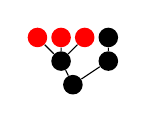
\begin{tikzpicture}[scale=.2]
\node[circle, scale=0.75, fill] (tid0) at (3,0){};
\node[circle, scale=0.75, fill] (tid1) at (2.25,1.5){};
\node[circle, scale=0.75, fill, red] (tid3) at (0.75,3){};
\node[circle, scale=0.75, fill, red] (tid4) at (2.25,3){};
\node[circle, scale=0.75, fill, red] (tid5) at (3.75,3){};
\draw[](tid1) -- (tid3);
\draw[](tid1) -- (tid4);
\draw[](tid1) -- (tid5);
\node[circle, scale=0.75, fill] (tid2) at (5.25,1.5){};
\node[circle, scale=0.75, fill] (tid6) at (5.25,3){};
\draw[](tid2) -- (tid6);
\draw[](tid0) -- (tid1);
\draw[](tid0) -- (tid2);

\end{tikzpicture}
\nodepart{two}
\footnotesize{4.38889}
\nodepart{three}
\footnotesize{$1$}
};
\node[draw opacity=0, fill opacity=0, anchor=south west] (dummyL) at (-18, -45){};
\node[draw=black, rectangle split, anchor=south west, rectangle split parts=3] (sn0xb39560) at ([xshift=2cm]sn0xb3be30.south east){
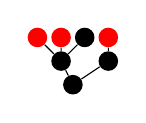
\begin{tikzpicture}[scale=.2]
\node[circle, scale=0.75, fill] (tid0) at (3,0){};
\node[circle, scale=0.75, fill] (tid1) at (2.25,1.5){};
\node[circle, scale=0.75, fill, red] (tid3) at (0.75,3){};
\node[circle, scale=0.75, fill, red] (tid4) at (2.25,3){};
\node[circle, scale=0.75, fill] (tid5) at (3.75,3){};
\draw[](tid1) -- (tid3);
\draw[](tid1) -- (tid4);
\draw[](tid1) -- (tid5);
\node[circle, scale=0.75, fill] (tid2) at (5.25,1.5){};
\node[circle, scale=0.75, fill, red] (tid6) at (5.25,3){};
\draw[](tid2) -- (tid6);
\draw[](tid0) -- (tid1);
\draw[](tid0) -- (tid2);

\end{tikzpicture}
\nodepart{two}
\footnotesize{4.37037}
\nodepart{three}
\footnotesize{$67\:33$}
};
\node[draw opacity=0, fill opacity=0, anchor=south west] (dummyL) at (-18, -45){};
\node[draw=black, rectangle split, anchor=south west, rectangle split parts=3] (sn0xb36480) at ([xshift=2cm]sn0xb39560.south east){
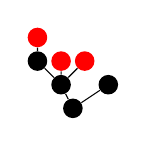
\begin{tikzpicture}[scale=.2]
\node[circle, scale=0.75, fill] (tid0) at (3,0){};
\node[circle, scale=0.75, fill] (tid1) at (2.25,1.5){};
\node[circle, scale=0.75, fill] (tid3) at (0.75,3){};
\node[circle, scale=0.75, fill, red] (tid6) at (0.75,4.5){};
\draw[](tid3) -- (tid6);
\node[circle, scale=0.75, fill, red] (tid4) at (2.25,3){};
\node[circle, scale=0.75, fill, red] (tid5) at (3.75,3){};
\draw[](tid1) -- (tid3);
\draw[](tid1) -- (tid4);
\draw[](tid1) -- (tid5);
\node[circle, scale=0.75, fill] (tid2) at (5.25,1.5){};
\draw[](tid0) -- (tid1);
\draw[](tid0) -- (tid2);

\end{tikzpicture}
\nodepart{two}
\footnotesize{4.56482}
\nodepart{three}
\footnotesize{$67\:33$}
};
\node[draw opacity=0, fill opacity=0, anchor=south west] (dummyL) at (-15, -60){};
\node[draw=black, rectangle split, anchor=south west, rectangle split parts=3] (sn0xb37640) at ([xshift=2cm]dummyL){
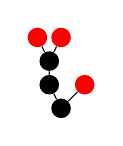
\begin{tikzpicture}[scale=.2]
\node[circle, scale=0.75, fill] (tid0) at (2.25,0){};
\node[circle, scale=0.75, fill] (tid1) at (1.5,1.5){};
\node[circle, scale=0.75, fill] (tid3) at (1.5,3){};
\node[circle, scale=0.75, fill, red] (tid4) at (0.75,4.5){};
\node[circle, scale=0.75, fill, red] (tid5) at (2.25,4.5){};
\draw[](tid3) -- (tid4);
\draw[](tid3) -- (tid5);
\draw[](tid1) -- (tid3);
\node[circle, scale=0.75, fill, red] (tid2) at (3.75,1.5){};
\draw[](tid0) -- (tid1);
\draw[](tid0) -- (tid2);

\end{tikzpicture}
\nodepart{two}
\footnotesize{4.58333}
\nodepart{three}
\footnotesize{$33\:67$}
};
\node[draw opacity=0, fill opacity=0, anchor=south west] (dummyL) at (-15, -60){};
\node[draw=black, rectangle split, anchor=south west, rectangle split parts=3] (sn0xb3a5d0) at ([xshift=2cm]sn0xb37640.south east){
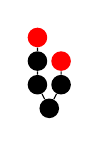
\begin{tikzpicture}[scale=.2]
\node[circle, scale=0.75, fill] (tid0) at (1.5,0){};
\node[circle, scale=0.75, fill] (tid1) at (0.75,1.5){};
\node[circle, scale=0.75, fill] (tid3) at (0.75,3){};
\node[circle, scale=0.75, fill, red] (tid5) at (0.75,4.5){};
\draw[](tid3) -- (tid5);
\draw[](tid1) -- (tid3);
\node[circle, scale=0.75, fill] (tid2) at (2.25,1.5){};
\node[circle, scale=0.75, fill, red] (tid4) at (2.25,3){};
\draw[](tid2) -- (tid4);
\draw[](tid0) -- (tid1);
\draw[](tid0) -- (tid2);

\end{tikzpicture}
\nodepart{two}
\footnotesize{4.4375}
\nodepart{three}
\footnotesize{$50\:50$}
};
\node[draw opacity=0, fill opacity=0, anchor=south west] (dummyL) at (-15, -60){};
\node[draw=black, rectangle split, anchor=south west, rectangle split parts=3] (sn0xb36010) at ([xshift=2cm]sn0xb3a5d0.south east){
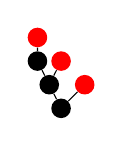
\begin{tikzpicture}[scale=.2]
\node[circle, scale=0.75, fill] (tid0) at (2.25,0){};
\node[circle, scale=0.75, fill] (tid1) at (1.5,1.5){};
\node[circle, scale=0.75, fill] (tid3) at (0.75,3){};
\node[circle, scale=0.75, fill, red] (tid5) at (0.75,4.5){};
\draw[](tid3) -- (tid5);
\node[circle, scale=0.75, fill, red] (tid4) at (2.25,3){};
\draw[](tid1) -- (tid3);
\draw[](tid1) -- (tid4);
\node[circle, scale=0.75, fill, red] (tid2) at (3.75,1.5){};
\draw[](tid0) -- (tid1);
\draw[](tid0) -- (tid2);

\end{tikzpicture}
\nodepart{two}
\footnotesize{4.34722}
\nodepart{three}
\footnotesize{$33\:33\:33$}
};
\node[draw opacity=0, fill opacity=0, anchor=south west] (dummyL) at (-15, -60){};
\node[draw=black, rectangle split, anchor=south west, rectangle split parts=3] (sn0xb3a370) at ([xshift=2cm]sn0xb36010.south east){
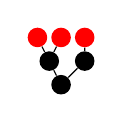
\begin{tikzpicture}[scale=.2]
\node[circle, scale=0.75, fill] (tid0) at (2.25,0){};
\node[circle, scale=0.75, fill] (tid1) at (1.5,1.5){};
\node[circle, scale=0.75, fill, red] (tid3) at (0.75,3){};
\node[circle, scale=0.75, fill, red] (tid4) at (2.25,3){};
\draw[](tid1) -- (tid3);
\draw[](tid1) -- (tid4);
\node[circle, scale=0.75, fill] (tid2) at (3.75,1.5){};
\node[circle, scale=0.75, fill, red] (tid5) at (3.75,3){};
\draw[](tid2) -- (tid5);
\draw[](tid0) -- (tid1);
\draw[](tid0) -- (tid2);

\end{tikzpicture}
\nodepart{two}
\footnotesize{4.05556}
\nodepart{three}
\footnotesize{$67\:33$}
};
\node[draw opacity=0, fill opacity=0, anchor=south west] (dummyL) at (-15, -60){};
\node[draw=black, rectangle split, anchor=south west, rectangle split parts=3] (sn0xb39de0) at ([xshift=2cm]sn0xb3a370.south east){
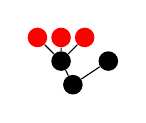
\begin{tikzpicture}[scale=.2]
\node[circle, scale=0.75, fill] (tid0) at (3,0){};
\node[circle, scale=0.75, fill] (tid1) at (2.25,1.5){};
\node[circle, scale=0.75, fill, red] (tid3) at (0.75,3){};
\node[circle, scale=0.75, fill, red] (tid4) at (2.25,3){};
\node[circle, scale=0.75, fill, red] (tid5) at (3.75,3){};
\draw[](tid1) -- (tid3);
\draw[](tid1) -- (tid4);
\draw[](tid1) -- (tid5);
\node[circle, scale=0.75, fill] (tid2) at (5.25,1.5){};
\draw[](tid0) -- (tid1);
\draw[](tid0) -- (tid2);

\end{tikzpicture}
\nodepart{two}
\footnotesize{4}
\nodepart{three}
\footnotesize{$1$}
};
\node[draw opacity=0, fill opacity=0, anchor=south west] (dummyL) at (-15, -75){};
\node[draw=black, rectangle split, anchor=south west, rectangle split parts=3] (sn0xb37bd0) at ([xshift=2cm]dummyL){
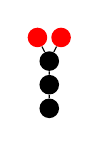
\begin{tikzpicture}[scale=.2]
\node[circle, scale=0.75, fill] (tid0) at (1.5,0){};
\node[circle, scale=0.75, fill] (tid1) at (1.5,1.5){};
\node[circle, scale=0.75, fill] (tid2) at (1.5,3){};
\node[circle, scale=0.75, fill, red] (tid3) at (0.75,4.5){};
\node[circle, scale=0.75, fill, red] (tid4) at (2.25,4.5){};
\draw[](tid2) -- (tid3);
\draw[](tid2) -- (tid4);
\draw[](tid1) -- (tid2);
\draw[](tid0) -- (tid1);

\end{tikzpicture}
\nodepart{two}
\footnotesize{4.5}
\nodepart{three}
\footnotesize{$1$}
};
\node[draw opacity=0, fill opacity=0, anchor=south west] (dummyL) at (-15, -75){};
\node[draw=black, rectangle split, anchor=south west, rectangle split parts=3] (sn0xb37750) at ([xshift=2cm]sn0xb37bd0.south east){
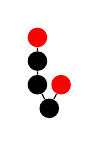
\begin{tikzpicture}[scale=.2]
\node[circle, scale=0.75, fill] (tid0) at (1.5,0){};
\node[circle, scale=0.75, fill] (tid1) at (0.75,1.5){};
\node[circle, scale=0.75, fill] (tid3) at (0.75,3){};
\node[circle, scale=0.75, fill, red] (tid4) at (0.75,4.5){};
\draw[](tid3) -- (tid4);
\draw[](tid1) -- (tid3);
\node[circle, scale=0.75, fill, red] (tid2) at (2.25,1.5){};
\draw[](tid0) -- (tid1);
\draw[](tid0) -- (tid2);

\end{tikzpicture}
\nodepart{two}
\footnotesize{4.125}
\nodepart{three}
\footnotesize{$50\:50$}
};
\node[draw opacity=0, fill opacity=0, anchor=south west] (dummyL) at (-15, -75){};
\node[draw=black, rectangle split, anchor=south west, rectangle split parts=3] (sn0xb3b350) at ([xshift=2cm]sn0xb37750.south east){
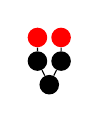
\begin{tikzpicture}[scale=.2]
\node[circle, scale=0.75, fill] (tid0) at (1.5,0){};
\node[circle, scale=0.75, fill] (tid1) at (0.75,1.5){};
\node[circle, scale=0.75, fill, red] (tid3) at (0.75,3){};
\draw[](tid1) -- (tid3);
\node[circle, scale=0.75, fill] (tid2) at (2.25,1.5){};
\node[circle, scale=0.75, fill, red] (tid4) at (2.25,3){};
\draw[](tid2) -- (tid4);
\draw[](tid0) -- (tid1);
\draw[](tid0) -- (tid2);

\end{tikzpicture}
\nodepart{two}
\footnotesize{3.75}
\nodepart{three}
\footnotesize{$1$}
};
\node[draw opacity=0, fill opacity=0, anchor=south west] (dummyL) at (-15, -75){};
\node[draw=black, rectangle split, anchor=south west, rectangle split parts=3] (sn0xb38ac0) at ([xshift=2cm]sn0xb3b350.south east){
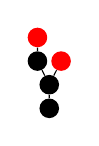
\begin{tikzpicture}[scale=.2]
\node[circle, scale=0.75, fill] (tid0) at (1.5,0){};
\node[circle, scale=0.75, fill] (tid1) at (1.5,1.5){};
\node[circle, scale=0.75, fill] (tid2) at (0.75,3){};
\node[circle, scale=0.75, fill, red] (tid4) at (0.75,4.5){};
\draw[](tid2) -- (tid4);
\node[circle, scale=0.75, fill, red] (tid3) at (2.25,3){};
\draw[](tid1) -- (tid2);
\draw[](tid1) -- (tid3);
\draw[](tid0) -- (tid1);

\end{tikzpicture}
\nodepart{two}
\footnotesize{4.25}
\nodepart{three}
\footnotesize{$50\:50$}
};
\node[draw opacity=0, fill opacity=0, anchor=south west] (dummyL) at (-15, -75){};
\node[draw=black, rectangle split, anchor=south west, rectangle split parts=3] (sn0xb38e80) at ([xshift=2cm]sn0xb38ac0.south east){
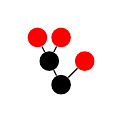
\begin{tikzpicture}[scale=.2]
\node[circle, scale=0.75, fill] (tid0) at (2.25,0){};
\node[circle, scale=0.75, fill] (tid1) at (1.5,1.5){};
\node[circle, scale=0.75, fill, red] (tid3) at (0.75,3){};
\node[circle, scale=0.75, fill, red] (tid4) at (2.25,3){};
\draw[](tid1) -- (tid3);
\draw[](tid1) -- (tid4);
\node[circle, scale=0.75, fill, red] (tid2) at (3.75,1.5){};
\draw[](tid0) -- (tid1);
\draw[](tid0) -- (tid2);

\end{tikzpicture}
\nodepart{two}
\footnotesize{3.66667}
\nodepart{three}
\footnotesize{$67\:33$}
};
\node[draw opacity=0, fill opacity=0, anchor=south west] (dummyL) at (-9, -90){};
\node[draw=black, rectangle split, anchor=south west, rectangle split parts=3] (sn0xb37e70) at ([xshift=2cm]dummyL){
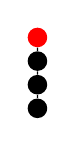
\begin{tikzpicture}[scale=.2]
\node[circle, scale=0.75, fill] (tid0) at (0.75,0){};
\node[circle, scale=0.75, fill] (tid1) at (0.75,1.5){};
\node[circle, scale=0.75, fill] (tid2) at (0.75,3){};
\node[circle, scale=0.75, fill, red] (tid3) at (0.75,4.5){};
\draw[](tid2) -- (tid3);
\draw[](tid1) -- (tid2);
\draw[](tid0) -- (tid1);

\end{tikzpicture}
\nodepart{two}
\footnotesize{4}
\nodepart{three}
\footnotesize{$1$}
};
\node[draw opacity=0, fill opacity=0, anchor=south west] (dummyL) at (-9, -90){};
\node[draw=black, rectangle split, anchor=south west, rectangle split parts=3] (sn0xb38160) at ([xshift=2cm]sn0xb37e70.south east){
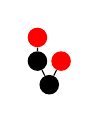
\begin{tikzpicture}[scale=.2]
\node[circle, scale=0.75, fill] (tid0) at (1.5,0){};
\node[circle, scale=0.75, fill] (tid1) at (0.75,1.5){};
\node[circle, scale=0.75, fill, red] (tid3) at (0.75,3){};
\draw[](tid1) -- (tid3);
\node[circle, scale=0.75, fill, red] (tid2) at (2.25,1.5){};
\draw[](tid0) -- (tid1);
\draw[](tid0) -- (tid2);

\end{tikzpicture}
\nodepart{two}
\footnotesize{3.25}
\nodepart{three}
\footnotesize{$50\:50$}
};
\node[draw opacity=0, fill opacity=0, anchor=south west] (dummyL) at (-9, -90){};
\node[draw=black, rectangle split, anchor=south west, rectangle split parts=3] (sn0xb39450) at ([xshift=2cm]sn0xb38160.south east){
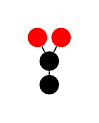
\begin{tikzpicture}[scale=.2]
\node[circle, scale=0.75, fill] (tid0) at (1.5,0){};
\node[circle, scale=0.75, fill] (tid1) at (1.5,1.5){};
\node[circle, scale=0.75, fill, red] (tid2) at (0.75,3){};
\node[circle, scale=0.75, fill, red] (tid3) at (2.25,3){};
\draw[](tid1) -- (tid2);
\draw[](tid1) -- (tid3);
\draw[](tid0) -- (tid1);

\end{tikzpicture}
\nodepart{two}
\footnotesize{3.5}
\nodepart{three}
\footnotesize{$1$}
};
\node[draw opacity=0, fill opacity=0, anchor=south west] (dummyL) at (-6, -105){};
\node[draw=black, rectangle split, anchor=south west, rectangle split parts=3] (sn0xb37f40) at ([xshift=2cm]dummyL){
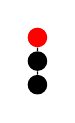
\begin{tikzpicture}[scale=.2]
\node[circle, scale=0.75, fill] (tid0) at (0.75,0){};
\node[circle, scale=0.75, fill] (tid1) at (0.75,1.5){};
\node[circle, scale=0.75, fill, red] (tid2) at (0.75,3){};
\draw[](tid1) -- (tid2);
\draw[](tid0) -- (tid1);

\end{tikzpicture}
\nodepart{two}
\footnotesize{3}
\nodepart{three}
\footnotesize{$1$}
};
\node[draw opacity=0, fill opacity=0, anchor=south west] (dummyL) at (-6, -105){};
\node[draw=black, rectangle split, anchor=south west, rectangle split parts=3] (sn0xb385b0) at ([xshift=2cm]sn0xb37f40.south east){

\begin{tikzpicture}[scale=.2]
\node[circle, scale=0.75, fill] (tid0) at (1.5,0){};
\node[circle, scale=0.75, fill, red] (tid1) at (0.75,1.5){};
\node[circle, scale=0.75, fill, red] (tid2) at (2.25,1.5){};
\draw[](tid0) -- (tid1);
\draw[](tid0) -- (tid2);

\end{tikzpicture}
\nodepart{two}
\footnotesize{2.5}
\nodepart{three}
\footnotesize{$1$}
};
\draw (sn0xb34100.south) -- (sn0xb3b0e0.north);
\draw (sn0xb34100.south) -- (sn0xb3bba0.north);
\draw (sn0xb34100.south) -- (sn0xb3b620.north);
\draw (sn0xb34100.south) -- (sn0xb36610.north);
\draw (sn0xb3b0e0.south) -- (sn0xb3c5d0.north);
\draw (sn0xb3b0e0.south) -- (sn0xb3a170.north);
\draw (sn0xb3bba0.south) -- (sn0xb36e20.north);
\draw (sn0xb3bba0.south) -- (sn0xb3a170.north);
\draw (sn0xb3b620.south) -- (sn0xb3a170.north);
\draw (sn0xb3b620.south) -- (sn0xb3be30.north);
\draw (sn0xb3b620.south) -- (sn0xb39560.north);
\draw (sn0xb36610.south) -- (sn0xb3a170.north);
\draw (sn0xb36610.south) -- (sn0xb36480.north);
\draw (sn0xb36610.south) -- (sn0xb39560.north);
\draw (sn0xb3c5d0.south) -- (sn0xb37640.north);
\draw (sn0xb3c5d0.south) -- (sn0xb3a5d0.north);
\draw (sn0xb3a170.south) -- (sn0xb3a5d0.north);
\draw (sn0xb3a170.south) -- (sn0xb36010.north);
\draw (sn0xb3a170.south) -- (sn0xb3a370.north);
\draw (sn0xb36e20.south) -- (sn0xb37640.north);
\draw (sn0xb36e20.south) -- (sn0xb36010.north);
\draw (sn0xb3be30.south) -- (sn0xb3a370.north);
\draw (sn0xb39560.south) -- (sn0xb3a370.north);
\draw (sn0xb39560.south) -- (sn0xb39de0.north);
\draw (sn0xb36480.south) -- (sn0xb36010.north);
\draw (sn0xb36480.south) -- (sn0xb39de0.north);
\draw (sn0xb37640.south) -- (sn0xb37bd0.north);
\draw (sn0xb37640.south) -- (sn0xb37750.north);
\draw (sn0xb3a5d0.south) -- (sn0xb37750.north);
\draw (sn0xb3a5d0.south) -- (sn0xb3b350.north);
\draw (sn0xb36010.south) -- (sn0xb38ac0.north);
\draw (sn0xb36010.south) -- (sn0xb37750.north);
\draw (sn0xb36010.south) -- (sn0xb38e80.north);
\draw (sn0xb3a370.south) -- (sn0xb3b350.north);
\draw (sn0xb3a370.south) -- (sn0xb38e80.north);
\draw (sn0xb39de0.south) -- (sn0xb38e80.north);
\draw (sn0xb37bd0.south) -- (sn0xb37e70.north);
\draw (sn0xb37750.south) -- (sn0xb37e70.north);
\draw (sn0xb37750.south) -- (sn0xb38160.north);
\draw (sn0xb3b350.south) -- (sn0xb38160.north);
\draw (sn0xb38ac0.south) -- (sn0xb37e70.north);
\draw (sn0xb38ac0.south) -- (sn0xb39450.north);
\draw (sn0xb38e80.south) -- (sn0xb39450.north);
\draw (sn0xb38e80.south) -- (sn0xb38160.north);
\draw (sn0xb37e70.south) -- (sn0xb37f40.north);
\draw (sn0xb38160.south) -- (sn0xb37f40.north);
\draw (sn0xb38160.south) -- (sn0xb385b0.north);
\draw (sn0xb39450.south) -- (sn0xb37f40.north);
\end{tikzpicture}

%%% Local Variables:
%%% TeX-master: "thesis/thesis.tex"
%%% End: 

